\subsection{Performance comparison with iZ3 and MathSat}\label{performance_euf}

This section will discuss a parametrized problem 
which will allows to test 
our implementation and constrast the execution with 
other interpolant generation
algorithms from Z3 and MathSat.

\begin{lemma} \label{performance_test_lemma}
  Let $x$ be a constant and $f$ an unary function in the EUF language. 
  For every $n \in \mathbb{N}$ the following conjunction is unsatisfiable:
  \begin{equation*}
    f^n(x) = f^{n+1}(x), f^2(x) = x, f(x) \neq x
  \end{equation*}
  where $f^n(x)$ denotes de application of the function $f$ n-times
  to the constant $x$.
\end{lemma}

\begin{proof}
  Applying the congruence and transitive rules to the equation $f^2(x) = x$, 
  we can prove that for any number $n$ the two following equations hold:
  $x = f^{2n}(x)$ and $f(x) = f^{2n+1}(x)$.

  At this point we distinguish two cases for $n$:

  \begin{itemize}
    \item Case $n$ is even: Then $\exists m \in \mathbb{N} . n = 2m$.
      So by choosing $n = m$ to the above sequence
      and by the axiom $f^{2m}(x) = f^{2m+1}(x)$ we have that
      $x = f(x)$.
    \item Case $n$ is odd: Similarly to the previous reasoning, 
      we can also infer the equation $f^{2m+1}(x) = f^{2m+2}(x)$
      by congruence, so $x = f(x)$.
    \end{itemize}

    In both cases the equation $x = f(x)$ reaches contradiction with the
    disequality $x \neq f(x)$.
\end{proof}

The interpolation pair for our performance test 
is $(f^n(x) = f^{n+1}(x) \land f^2(x) = x \land f(a) \neq a, x = a)$
for fixed $n \in \mathbb{N}$.
It is easy to see that the pair is inconsistent due to the lemma 
\ref{performance_test_lemma}. 

By lemma \ref{performance_test_lemma}
we can also see that the formula $x = a \rightarrow \bot$ is an 
interpolating formula for all fixed $n$ in this parametrized problem.
We designed this problem because it is easy to verify the 
correctness of output of the algorithms and to measure 
the time used by the algorithms for large values of $n$. 
We executed instances of this problem for values of $n$
in the range $\{1, \dots, 10000\}$ using a computer desktop
equipped with an Intel i7-9700 @ 4.70 GHz and 16Gb of memory. 
The output produced by the interpolant generation algorithms
were the expected formula.
The following graph reports the time measured by the UNIX
utility $times$ of our implementation, iZ3, and the interpolation 
generation algorithm from Mathsat.

\begin{figure}
  \centering
  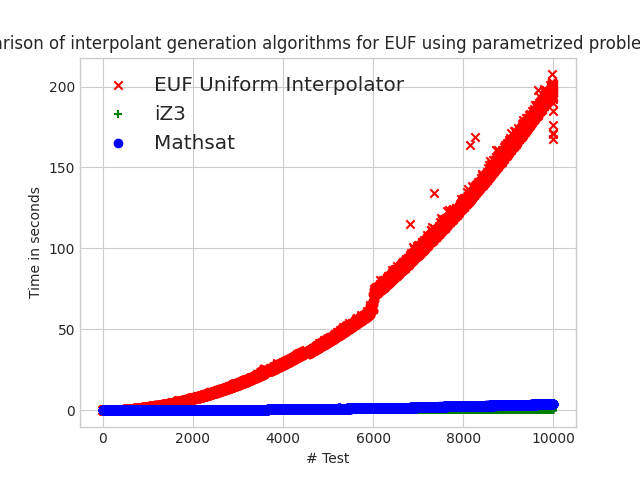
\includegraphics[scale=0.9]{figures/eufi_performance_graph}
  \caption{Performance comparison graph of EUF interpolant generation
  algorithms for paramatrized problem from section \ref{performance_euf}} 
  \label{performance_graph_euf}
\end{figure}

We noticed a quadractic behaviour in the graph for the time 
required by our implementation
and a linear behaviour by iZ3 and Mathsat. However, 
according to the following polynomial 
fitting computation, 
we noticed that for the case of our implementation, 
a linear fitting obtained a smaller 
quadratic error compared to the quadratic fitting;  
for the case of the Mathsat
results, a quadratic fitting obtained a smaller 
quadratic errror.

\begin{table}[h]
  \centering
  \begin{tabular}{ccc}
    \toprule
    {}                 & Error of linear fitting & Error of quadratic fitting \\
    \cmidrule{2-2} \cmidrule{3-3} \\
    iZ3                &  1.8723744548656934e-27 & 2.3456535579201815e-26     \\
    Mathsat            &  8.690566310635247e-23  & 7.576220133742597e-23      \\
    Our implementation &  2.5622746654442585e-20 & 6.648236698726508e-20      \\
    \bottomrule
  \end{tabular}
  \caption{Table of polynomial fitting errors of degrees 1, 2 for the
  EUF experiments of section \ref{performance_euf}.}
\end{table}

%%% Local Variables:
%%% mode: latex
%%% TeX-master: "main"
%%% End:
